%!TeX root=../tese.tex
%("dica" para o editor de texto: este arquivo é parte de um documento maior)
% para saber mais: https://tex.stackexchange.com/q/78101

\chapter{An imaginary function extraction plugin}

Although every modern IDE has a series of tools for automating common simple code refactorings, the automation of suggestions of refactorings is still lacking. E.g., renaming a variable can be easily accomplished by tools that scan your program for instances of this variable in the appropriate scope. But there is no efficient tool to our knowledge that automatically detects the need to rename a variable and suggests a new name.

In this chapter we will propose the structure of how one could create an IDE plugin that automates refactorings of the function extraction type and suggests instances of such refactorings. Our objective is by no means the construction nor the implementation of this imaginary plugin, as previously stated in our goals we only intend to create a model that, given only a function definition, is capable of performing a function extraction. We propose this plugin as a mental exercise to clarify some of the practical uses of the work proposed in this project and as a way to introduce software engineering concepts that the readers may need to fully comprehend to understand this project.






\section{Code Refactoring}

This project aims at automating refactorings but we never actually defined what refactoring is, so let us look at some definitions starting with the one who coined the term:

\begin{myquote}
    
\textit{This thesis defines a set of program restructuring operations (refactorings) that support the design, evolution and reuse of object-oriented application frameworks. [...] The refactorings are defined to be behavior preserving, provided that their preconditions are met. Most of the refactorings are simple to implement and it is almost trivial to show that they are behavior preserving.}\\ \citet{opdyke1992refactoring}
\end{myquote}

Another simpler definition from another pioneer on the subject, Martin Fowler, could be useful to those new to the term:

\begin{myquote}
\textbf{Refactoring} (noun): \textit{a change made to the internal structure of software to make it easier to understand and cheaper to modify without changing its observable behavior.} \\\citet{martinfowler}
\end{myquote}
\begin{myquote}
\textbf{Refactoring} (verb): \textit{to restructure software by applying a series of refactorings without changing its observable behavior.} \\\citet{martinfowler}
\end{myquote}


From these definitions we can gather that ideally each refactoring would be a simple and small step that a programmer could take in order to improve the perceived complexity of a program and be more compliant with best practices. After taking a series of these small steps a program will have an improved maintainability, being more readable and easier to debug while behaving the same exact way. Fig.~\ref{ilustracao_refac_func2class} shows an example of such an operation, a refactoring categorized as \textit{Combine Functions into Class}.

\begin{figure}[!ht]
\centerline{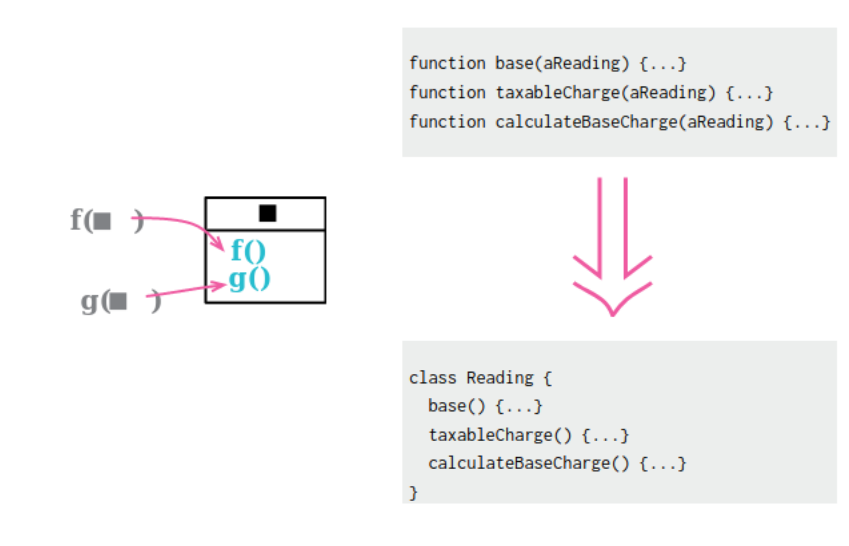
\includegraphics[width=0.8\textwidth]{figuras/class_extract.png}   }
\caption{An instance of the ``Combine Functions into Class'' refactoring. Example extracted from  \citep{martinfowler}.}
\label{ilustracao_refac_func2class}
\end{figure}


However, in practice this definition of refactoring being a behavior-preserving code transformation does not always hold true. It is not uncommon to use the term refactoring in ways that defy its academic definition, Martin Fowler addresses this:



\begin{myquote}
\textit{Over the years, many people in the industry have taken to use `refactoring' to mean any kind of code cleanup---but the definitions above point to a particular approach to cleaning up code. Refactoring is all about applying small behavior-preserving steps and
making a big change by stringing together a sequence of these behavior-preserving steps. Each individual refactoring is either pretty small itself or a combination of small steps. As a result, when I'm refactoring, my code doesn't spend much time in a broken state, allowing me to stop at any moment even if I haven't finished.}
\\
\\
\textit{If someone says their code was broken for a couple of days while they are
refactoring, you can be pretty sure they were not refactoring.}\\\citet{martinfowler}
\end{myquote}








That is to say, colloquially refactoring is often used as something more generic and less rigorous than Opdyke's or Fowler's definitions.
A survey of 328 professional software engineers at Microsoft found that developers do not necessarily consider that refactoring is confined to behavior preserving transformations \citep{7vista}. Furthermore: \begin{myquote}
\textit{[...] 78\% define refactoring as code transformation that improves some aspects of program behavior
such as readability, maintainability, or performance. 46\%
of developers did not mention preservation of behavior,
semantics, or functionality in their refactoring definition
at all. [...]
The following shows a few examples of refactoring
definitions by developers.
\\
\qquad `Rewriting code to make it better in some way.'
\\
\qquad `Changing code to make it easier to maintain. Strictly
speaking, refactoring means that behavior does not change,
but realistically speaking, it usually is done while adding
features or fixing bugs.'} 
\\
\citet{7vista} \end{myquote}


Bearing in mind those different meanings, we will stick to Martin Fowler's definition unless stated otherwise. \citet{catalog} has a catalog where he defines many different types of refactorings but we are interested in automating a specific type of refactoring, the function extraction. When our hypothetical plugin suggests a function extraction to its fictional user it will only suggest the extraction, no feature will be added or subtracted. Further code improvements are out of the scope of this project and are left as possible paths for future work.





Following Martin Fowler's nomenclature system \citep{martinfowler}, in this project we will explore the \textit{function extraction} refactoring in particular, where a long function that does many tasks is broken down into smaller functions, that only do one simple task each, being called one after the other. Each new function created from the larger original one is an instance of a function extraction. It is not uncommon to have a series of function extractions being applied sequentially to a single large function. Fig.~\ref{img:func_exract} gives an example of this refactoring.


\begin{figure}[!ht]
\centerline{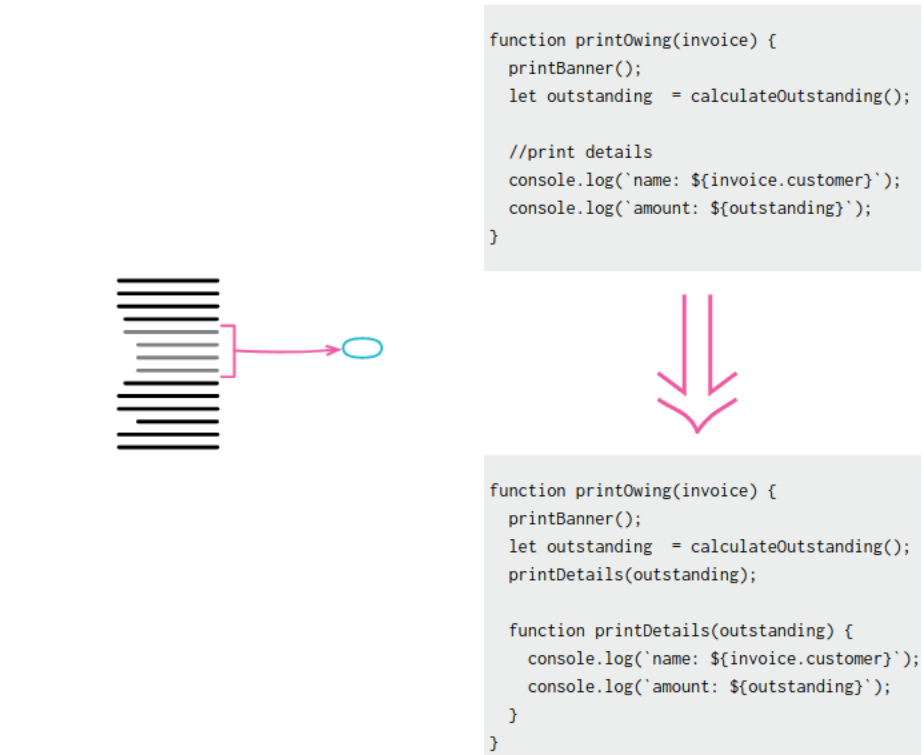
\includegraphics[width=0.8\textwidth]{figuras/func_extract.png}   }
\caption{An instance of the ``Function Extraction'' refactoring. Example extracted from  \citep{martinfowler}.}
\label{img:func_exract}
\end{figure}


\section{The Plugin}

With a clear definition of what is a refactoring and of our objectives we will explore our theoretical plugin and how it could be built. Fig.~\ref{img:plugin} presents the outline of how this plugin would work.

\begin{figure}[!ht]
\centerline{
\includegraphics[width=1.1\textwidth]{figuras/plugin.drawio.png}   }
\caption{Outline of our imaginary plugin broken down into three different parts.}
\label{img:plugin}
\end{figure}



\subsection{Detecting Refactoring Opportunities} 
\label{sec:code_metrics}

As previously stated, code refactoring is not a new subject, extensive work has already been done to classify different types of refactorings. Furthermore, there are no lack of tools \citep{bavote_smell,bavota_smell2,jdeodorant,dig_smells} to identify \textit{code smells} \citep{martinfowler}, a common pattern that may serve as an indication of a deeper problem in the way the system is structured and the need of refactoring. For example a really long function may indicate the need for a function extraction refactoring. 

There are many approaches one could take in order to identify refactoring opportunities. One approach could be to leverage said code smells and their vast literature, another way could be to construct heuristics utilizing a set of code complexity metrics.


There are quite a few metrics that aim at measuring the perceived complexity of a piece of code --- not in the sense of \textit{execution time complexity} but in the sense of \textit{readability and maintainability}. By looking solely at the source code, without executing it, it is possible to provide an estimation of the quality of the software. Some metrics can be more specific and restrictive in their use, for example being tailored to a single programming paradigm (e.g. this suite of metrics designed for Object Oriented programming \citep{OO_metrics}). Other metrics may try to identify ``code smells'' or be specific to a single programming language \citep{goreport}.


Which of these ideas is the best we cannot say without testing and the results would ultimately be dependent on the implementation of the heuristics, but since we are dealing with an imaginary plugin we are not concerned with such details. We will explore the simple code complexity metric known as \textit{maintainability index} in order to better illustrate this piece of our imaginary plugin.

In section ~\ref{sec:mauricio} we will see another possible approach that utilizes machine learning to detect refactoring opportunities and the refactoring type to be used.

\subsubsection{Cyclomatic complexity}
The cyclomatic complexity proposed in 1976 \citep{cyclomatic}, may be defined as the number of linearly independent paths within a piece of code. A program with no control flow statements (such as loops and conditionals) will have a cyclomatic complexity of 1, a program with one conditional statement $if$ will have cyclomatic complexity of 2, one independent path for a True $if$ statement and another for a False $if$ statement.
Cyclomatic complexity may be used as a bound for the number of necessary unit tests for $100\%$ code coverage and a high cyclomatic complexity may be an indicative of complex nested flow statements.


\subsubsection{Halstead Metrics}
The Halstead metrics where developed in 1977 \citep{halstead} as an attempt to define and analyze static properties of a given software, trying to capture a measure of how difficult it is to write or understand a given piece of code. They also estimate how many bugs are present in a given snippet of code.
Let,
\begin{itemize}
    \item[] $\eta_{1}=$ Number of distinct operators     
    \item[] $\eta_{2}=$ Number of distinct operands
    \item[] $N_{1}=$ Total number of operators
    \item[] $N_{2}=$ Total number of operands
\end{itemize}
Halstead defines volume, difficulty, effort and estimated number of bugs as:
\begin{itemize}
    \item[] $V = (N_{1} + N_{2}) * \lg (\eta_{1} + \eta_{2})$ 
    \item[] $D = \frac{\eta_{1}}{2} * \frac{N_{2}}{\eta_{2}} $
    \item[] $E = D*V$
    \item[] $\hat{B} = \frac{ E^{\frac{2}{3}} } {3000}  $
\end{itemize}

\subsubsection{Maintainability Index}
Throughout the years, the maintainability index formula has been tweaked and refined, but on the original paper \citep{maintainability_index} it was defined as:
$$ MI = 171 - 5.2 * \ln (V)  - 0.23 * G - 16.2 * \ln (LoC) $$
Where $V$ is the Halstead Volume, $G$ is the Cyclomatic Complexity and $LoC$ is the total number of lines of code.
Typical values for the maintainability index range from 0 to 100 with 0 being a hard to maintain code and 100 being a well structured, small and easy to maintain code.


\subsection{Refactoring Prediction}

This is the kernel of this plugin and also our main objective in this project. As such, let us treat it as a black box model that simply works until we arrive at Chapter~\ref{chap:models} where we will present our attempts at solving this problem. 


\subsection{Performing Refactorings}
\label{sec:lsp}

Language Server Protocol \citep{lsp}, or LSP as it is commonly referred, was introduced to address the duplication of effort and code across IDE's and text editors. The idea is to create a standard that allows a plugin for a given language (e.g. auto-completion for python) to work in any development tool (e.g. a plugin designed for Atom will work in VSCode) thus reducing the workload of language providers and tooling vendors. Fig~\ref{lsp_image} illustrates this idea.

\begin{figure}[!ht]
\centerline{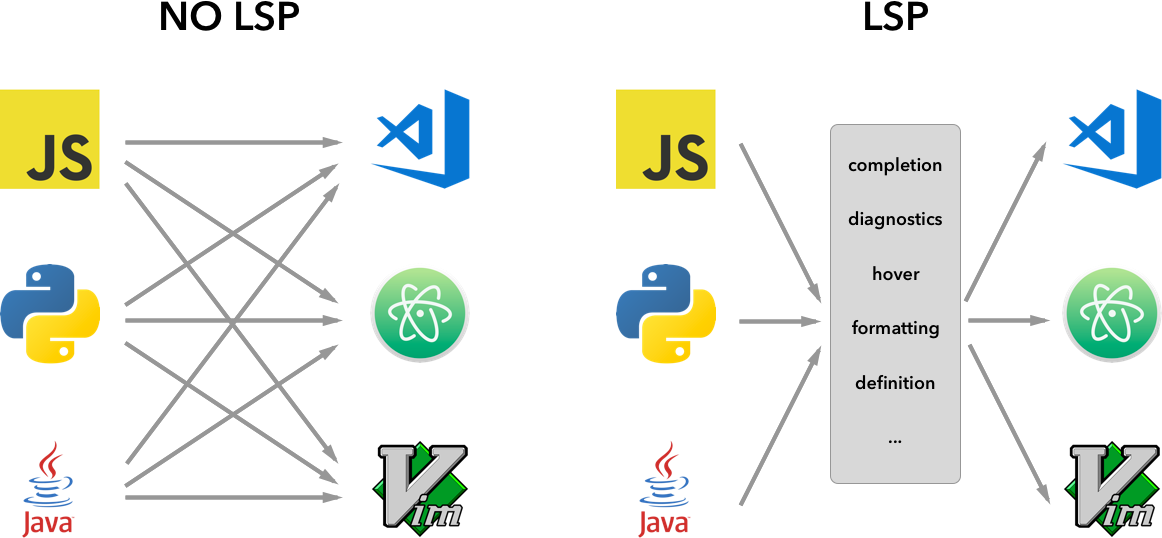
\includegraphics[scale=0.26]{figuras/lsp-ilustracao.png}   }
\caption{An illustration of the problem that LSP was designed to solve. Without LSP we have M languages that need to have support implemented in N different IDE's, but with LSP's we only need to implement support for a language once and it can be re-used anywhere \citep{lsp_ilustracao}.}
\label{lsp_image}
\end{figure}


The goal of LSP is to allow the implementation and distribution of support for a programming language without involving any particular text editor by standardizing  the interaction between the IDE's and the servers that provide language specific features.

With the use of a language server the function extraction refactoring could be easily accomplished by providing the line span to be extracted, in our particular case we could use the Eclipse JDT Language Server \citep{lsp_jdt} to potentially accomplish this for the Java programming language. By describing a refactoring in terms of operations done through the LSP the instructions generated by our model can be easily utilized in any development environment capable of communicating with a language server. It is important to note that function extractions are not always performed with a continuous set of lines which could prove itself a limitation for currently implemented LSP instructions, e.g. the Eclipse JDT Language Server expects a continuous line span. To perform more complex function extractions there may be a need to expand current LSP instruction sets.

